\chapter{The \textit{Java Privacy Guard}} \label{chapter:jpg}

In this chapter we give a overview of our implementation of the OpenPGP message format in Java. We show how we implemented the structures described in chapter \ref{chapter:messageformat}. We illustrate the structure of our implementation. Furthermore we give an introduction of our API. \\
%Additionally we discuss the implementation security and possible attacks.  \\


As practical part of this thesis an implementation of the OpenPGP message format \cite{RFC4880} in the \textit{Java} programing language was done. This created a library workingtitled \textbf{Java Privacy Guard}.

For cryptographic primitives like basic data types, encryption and digest algorithms we used the \myacro{IAIK-JCE} library. \\

The Packet- and Transferable-structure as described in chapter \ref{chapter:messageformat} represents the basic structure of our implementation. All Packets defined in \cite[section 5]{RFC4880} are implemented as one or more Java-classes. Additionally all relevant Packet-compositions are implemented in the form of Transferable-classes as defined in \cite[section 11]{RFC4880}. \\

Parsing and constructing of Transferables and other internal data processing heavily relies on Java's stream architecture. This allows a fast and memory-saving flow of data. \\

To facilitate the use of our implementation we crated two APIs for access to the library functionality. The APIs are explained in the section following.

\section{The APIs}

In this section we give an overview of our two APIs. We highlight the difference between the two APIs and describe how they implement the OpenPGP message format. Furthermore we show how the high-level API can be used to perform basic OpenPGP operations. Figure \ref{fig:transferablehierarchy} illustrates the structure of the high-level API. \\

The high-level API represents the interface used by users of our library. It mostly consists of Transferable-classes and related toolbox-classes.

The low-level API represents the inner working of the library. It consists of all Packet-classes. This API is used heavily in our implementation, specifically in the high-level API. Furthermore it is possible to use it for behavior not covered by the high-level API. Figure \ref{fig:packethierarchy} illustrates the structure of the low-level API.

\begin{figure}[p]
	\centering
	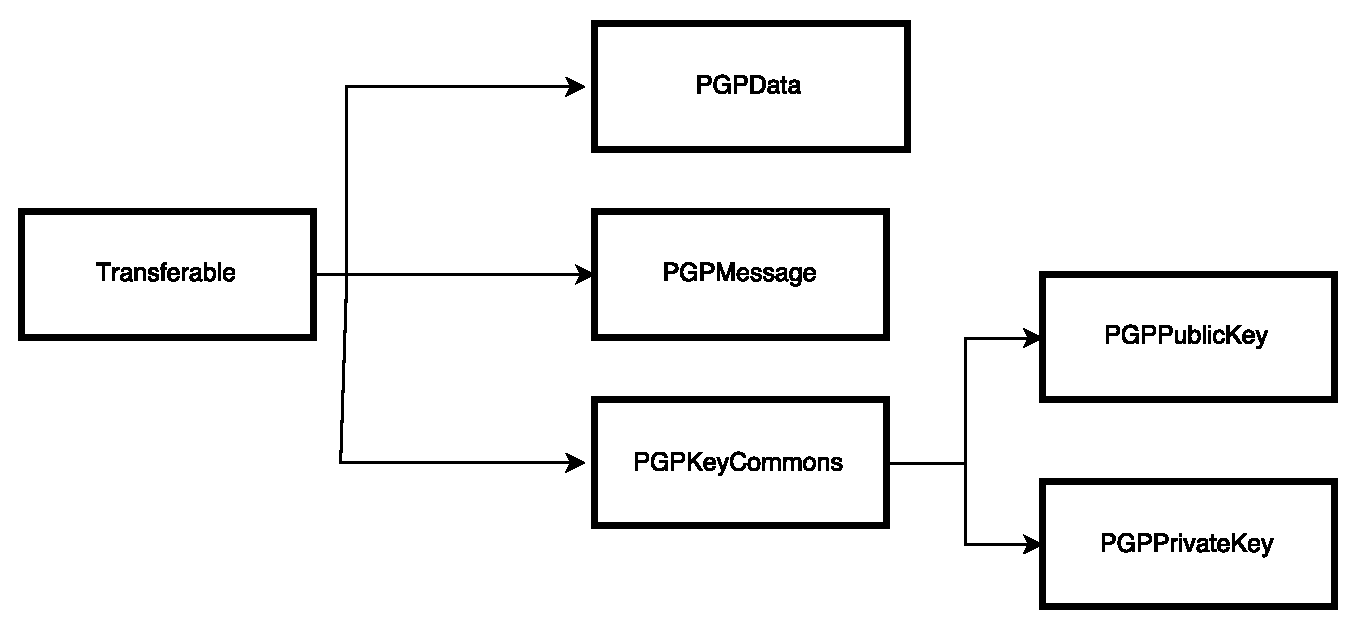
\includegraphics[width=1\linewidth]{figures/TransferableHierarchy.pdf}
	\caption[]{The high-level API: Transferable hierarchy }
	\label{fig:transferablehierarchy}
\end{figure}

\begin{figure}[p]
	\centering
	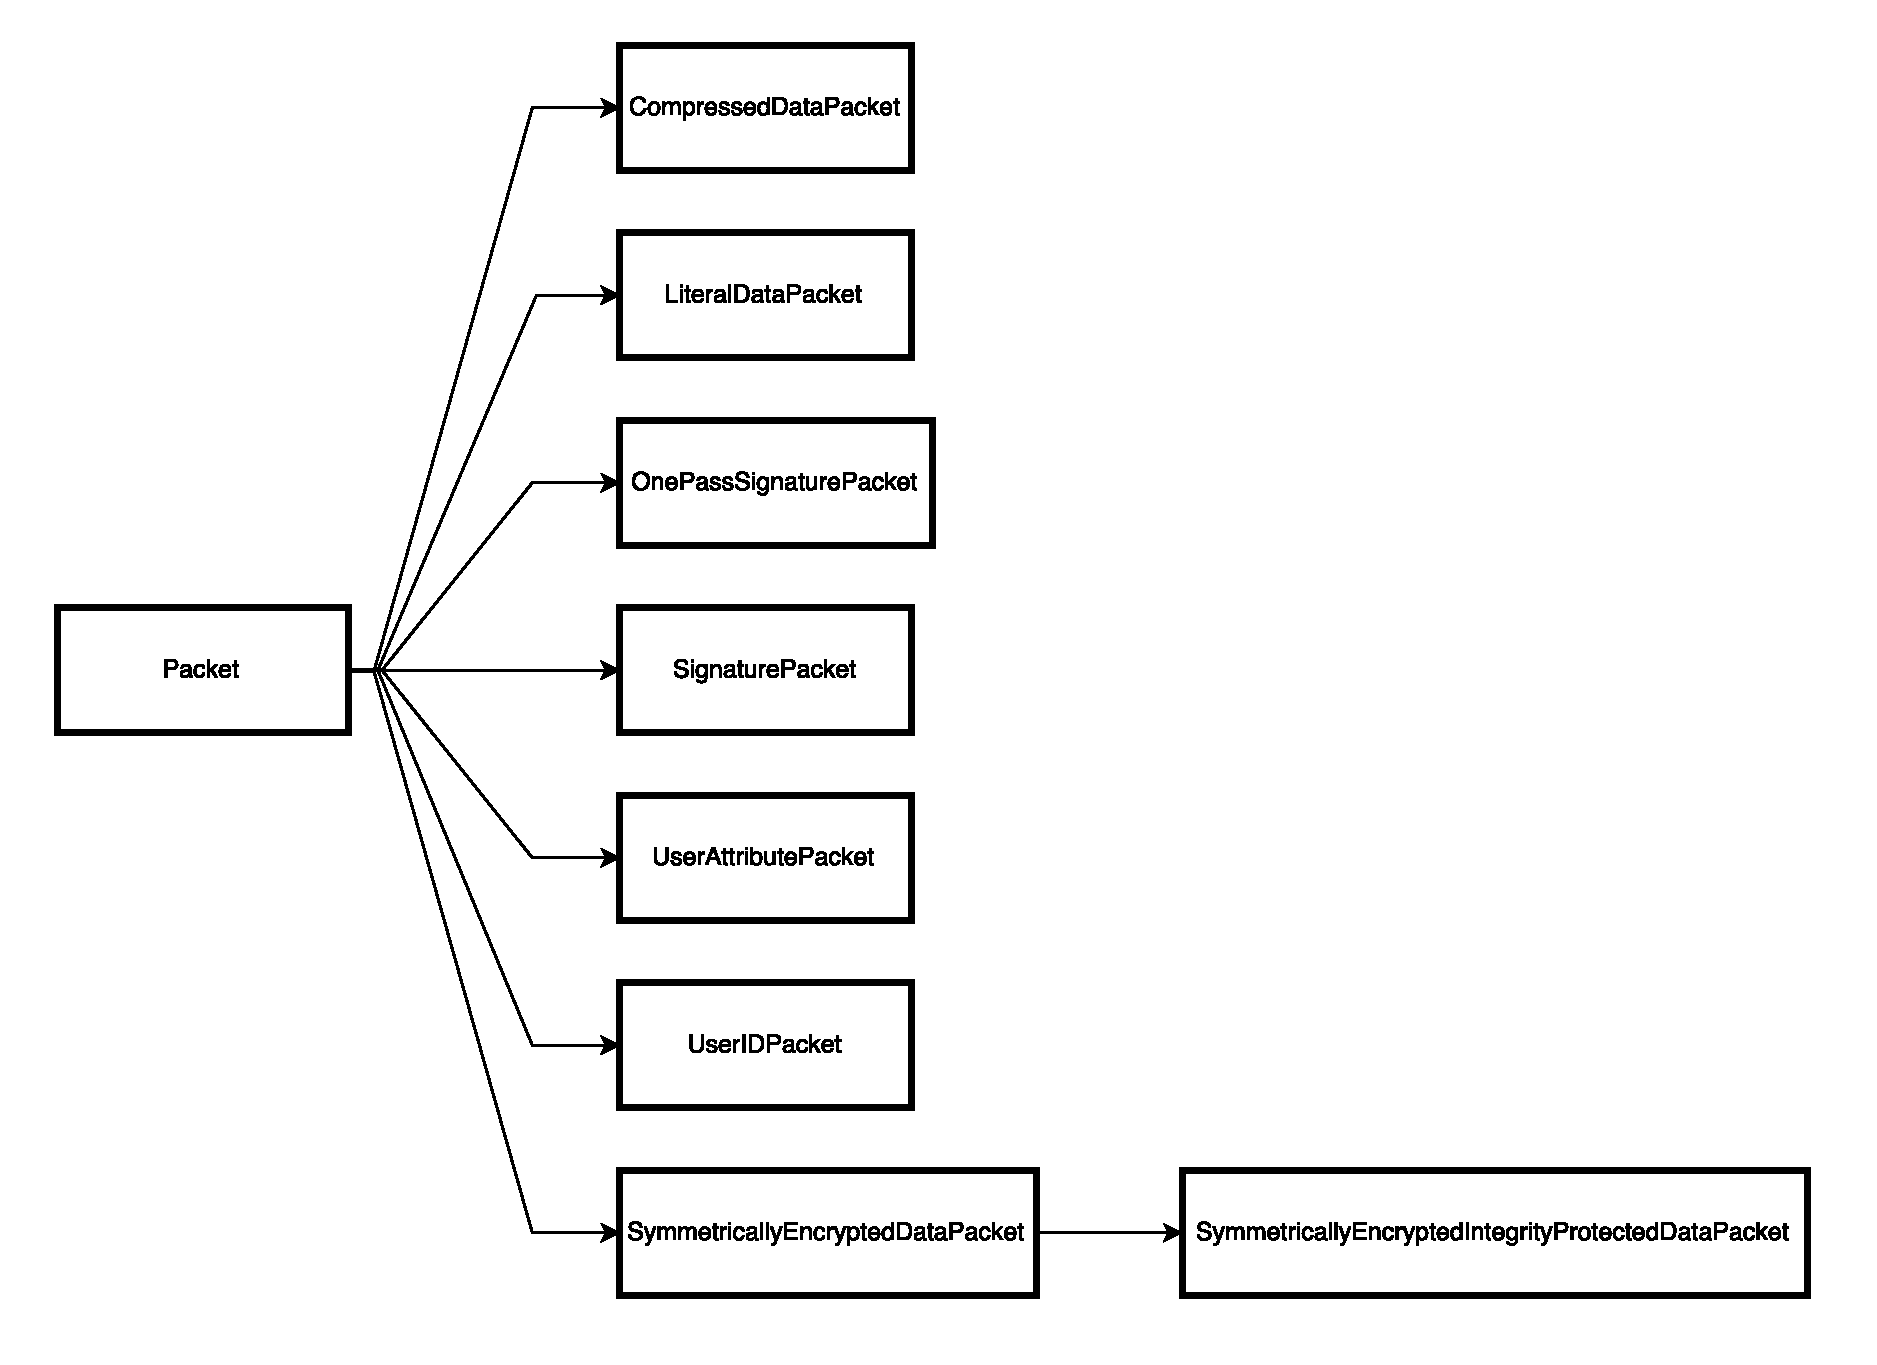
\includegraphics[width=1\linewidth]{figures/PacketHierarchy.pdf}
	\caption[]{The low-level API: Packet hierarchy }
	\label{fig:packethierarchy}
\end{figure}

To illustrate the functionality of the high-level API figure \ref{fig:jpg:key} shows how to load an OpenPGP key. In this example a keyring is loaded using the \textit{PGPReader} functionality. It automatically reads all keys from the file. In addition it builds the class-structure needed to work with the keys. Afterwards it is possible to retrieve a specific \textit{PGPKeyPair} identified by User ID.

Figure \ref{fig:jpg:enc} shows how to encrypt and sign data. First the demo data is stored in a byte array. This allows processing of generic data. Afterwards a \textit{PGPData} encrypter is created and configured. It is possible to encrypt the data for multiple keys. In addition the symmetric algorithm has to be configured. The used asymmetric algorithm is derived from the type of the \textit{PGPKeyPair} objects. Furthermore the signing process is configured.  In the end a \textit{PGPWriter} object is used to post-process the encrypted data. Thanks to Java's stream architecture it is possible to process the ciphertext or just store it.

% TODO figure --> lstlisting ?
\begin{figure}[p]
	\centering
	\lstinputlisting[style=myjava]{figures/KeyDemo.java}
	\caption{Loading an OpenPGP key using JavaPrivacyGuard}
	\label{fig:jpg:key}
\end{figure}

\begin{figure}[p]
	\centering
	\lstinputlisting[style=myjava]{figures/EncryptionDemo.java}
	\caption{Encrypting and signing data using JavaPrivacyGuard}
	\label{fig:jpg:enc}
\end{figure}


%\section{Issues during Implementation}
%
%\subsection{Unsigned and Java}
%
%\subsection{RFC}
%
%--- Ab hier section Evaluation? ---
%
%\section{Interoperability}
%
%\subsection{Bouncycastle}
%
%\subsection{GnuPG}

\newpage

\section{Implementation Security}
In this section, we give an overview of the security measures of our implementation. 
Security concerns, as long as they affect the actual design of the OpenPGP standard, are discussed in chapter \ref{chapter:concerns} and in \cite[section 14]{RFC4880}.  \\

Basic security measures like constant-time implementations are taken into account by our implementation. 

We use the \myacro{IAIK-JCE} toolbox to perform cryptographic operations and some other tasks. The toolbox is developed with a focus on security and well tested. No other external libraries are used. 

Another issue are weak defaults for ciphers and other algorithms. Because of the generic nature of a library our implementation does not set any defaults. Thus the issue of bad defaults is shifted to the user of the library. \\

%Since all OpenPGP implementations can be used as oracle [TODO schneier paper] it is recommended not to use OpenPGP in an unprotected and interactive mode. Due to the non-interactive nature of common applications (email) this was not taken into account.

%\todo{list attacks and show how our implementation reacts to it?}





